\begin{pa} \label{PA:4.1}
Suppose that a person is taking a walk along a long straight path and walks at a constant rate of 3 miles per hour.
\ba
	\item On the left-hand axes provided in Figure~\ref{F:4.1.PA1}, sketch a labeled graph of the velocity function $v(t) = 3$.  
\begin{figure}[h]
\begin{center}
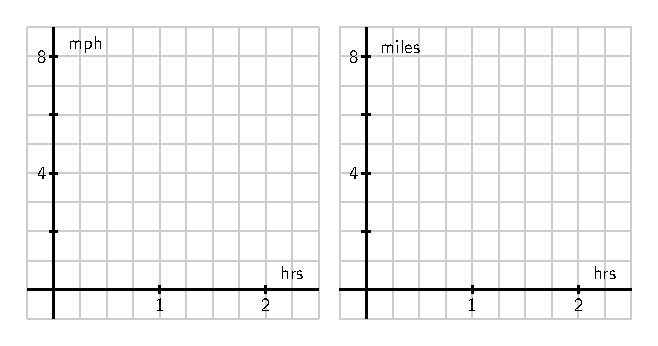
\includegraphics{figures/4_1_PA1.eps}
\caption{At left, axes for plotting $y = v(t)$; at right, for plotting $y = s(t)$.} \label{F:4.1.PA1}
\end{center}
\end{figure}
Note that while the scale on the two sets of axes is the same, the units on the right-hand axes differ from those on the left.  The right-hand axes will be used in question (d).
	\item How far did the person travel during the two hours?  How is this distance related to the area of a certain region under the graph of $y = v(t)$?
	\item Find an algebraic formula, $s(t)$, for the position of the person at time $t$, assuming that $s(0) = 0$.  Explain your thinking.
	\item On the right-hand axes provided in Figure~\ref{F:4.1.PA1}, sketch a labeled graph of the position function $y = s(t)$.
	\item For what values of $t$ is the position function $s$ increasing?  Explain why this is the case using relevant information about the velocity function $v$.
\ea
\end{pa} 
\afterpa